Let's take a region of space containing a number $N$ of nodes. This system can represent, for example, the hydraulic network of a city. 
For a node we define its ``energy'' flow $\varphi$ (in the case of the hydraulic network, what is flowing between the nodes is water). How much ``energy'' do we need to insert in the system? \\
If we have to distribute something to all the nodes, the most basic way to do it is to connect one on one all the nodes, as to form a long chain. \\
\begin{center}
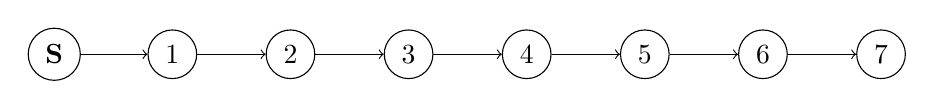
\begin{tikzpicture}[node distance={15mm}, main/.style = {draw,circle}]
\node[main] (1) {1};
\node[main] (0) [left of=1] {\textbf{S}};
\node[main] (2) [right of=1] {2};
\node[main] (3) [right of=2] {3};
\node[main] (4) [right of =3] {4};
\node[main] (5) [right of =4] {5};
\node[main] (6) [right of=5] {6};
\node[main] (7) [right of=6] {7};
\draw[->] (0) -- (1);
\draw[->] (1) -- (2);
\draw[->] (2) -- (3);
\draw[->] (3) -- (4);
\draw[->] (4) -- (5);
\draw[->] (5) -- (6);
\draw[->] (6) -- (7);
\end{tikzpicture}
\end{center}
If the flow out of the source $S$ is $\phi$, the flow after the first node is $\phi - \varphi$, and so on, and we expect that the flow arriving to the final node will be $\varphi$. \\
So the total energy is 
$$
	E_T \approx l\sum_{k=0}^{N-1} (\phi - k\varphi) = l\varphi\sum_{k=0}^{N-1} k`
$$
$$
	E_T \propto l\varphi N^2
$$
So the totaly energy that is required to provide for all the nodes, with this configuration, is proportional to the square of the total number of nodes. So with this configuration we have a network that is very easy to implement, but the network is very inefficient. \\ \\ 
Another possible connection of the nodes is the following one:
\begin{center}
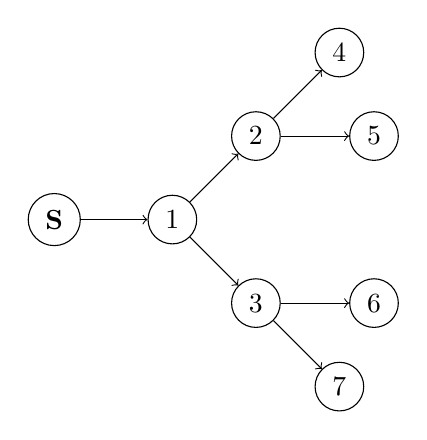
\begin{tikzpicture}[node distance={15mm}, main/.style = {draw,circle}]
\node[main] (1) {1};
\node[main] (0) [left of=1] {\textbf{S}};
\node[main] (2) [above right of=1] {2};
\node[main] (3) [below right of=1] {3};
\node[main] (4) [above right of =2] {4};
\node[main] (5) [right of =2] {5};
\node[main] (6) [right of=3] {6};
\node[main] (7) [below right of=3] {7};
\draw[->] (0) -- (1);
\draw[->] (1) -- (2);
\draw[->]  (1) -- (3);
\draw[->]  (2) -- (4);
\draw[->]  (2) -- (5);
\draw[->]  (3) -- (6);
\draw[->]  (3) -- (7);
\end{tikzpicture}
\end{center}
So each node is linked to two mode nodes. This is what is called a tree structure. \\
The main problem with such a structure is that the path between the nodes is always the same, but it is impossible to design a city in such a way. \\
The number of nodes is $N = 2^{m+1}$, where $m$ is the number of levels. \\
The relation for the flow in each level is
$$
	2\phi_k + \varphi = \phi_{k-1}
$$
where we assume again that the flow in the final level is $\varphi$. \\
$\phi_k$ then is
$$
	\phi_k = (2^{m+1-k}-1)\varphi
$$
Then:
$$
	E_T = d\varphi\sum_{k=1}^m 2^k(2^{m+1-k}-1) \approx d\varphi m 2^{m+1}	
$$
$$
	E_T = d\varphi N \log_2N
$$
This configuration is much more efficient than the previous alternative, although it is impossible to put to practice. \\ \\ 
So we need to find a solution that is in the middle of these two. \\ \\
Another possible structure consists of connecting all the nodes to the source, making a star network: also this model is of course impossible to put in practice. \\
However, in this case the total energy required is proportional to $NL$, where $L$ is the scale length of the system. 
$$
	E_T \propto NL
$$
The proportionality to $L$ is due to the fact that the average length of the links is proportional to the size of the space. \\
Since 
$$
	N = \left(\frac{L}{l} \right)^D
$$
where $D$ is the system dimension (e.g. 1D, 2D...).
We have that
$$
	E_T \propto N\overline{L} \approx N^{1+1/D} = V^{\frac{D+1}{D}}
$$
We notice that:
\begin{itemize}
	\item for a 2D system, like a city, $E \propto V^{\frac{3}{2}}$
	\item for a 3D system, like biological systems, $E \propto V^{\frac{4}{3}}$
\end{itemize}
In any case the exponent is greater than one so, soon or later, the system will collapse.
The problem is also logistic, because in a real transportation line there is also waste, that has to be disposed of. \\ \\
If we consider our system to be an animal's body, this would mean that in order to survive the amount of blood in its body must grow with the size by an amount of $4/3$. This would mean that very big animals can't survive, but they do, and the solution is in Kleiber's law. \\
As animals get bigger, their demand of energy goes down, so their metabolism slows down.  


Once we have a model (which hopefully is a good one), the model is deterministic, so if we know the initial conditions os the system, we know exactly what state the system will have at any future time. \\
The problem with this is that we don't know the initial conditions with absolute certainty. So at this point the question, that will be answered later, is: \\
How much error in the initial conditions is acceptable before that the previsions of our model start to diverge from the real evolution in an unacceptable way?